\documentclass{beamer}
\usepackage{graphicx}
\usepackage{helvet}
\title[Spatial Econophysics]{MPhys Project: Spatial Econophysics}
\author{Lawrence Mitchell}
\date{March 24, 2005}
\usetheme{Hannover}

\begin{document}

\frame
{
  \begin{minipage}[b]{0.75\textwidth}
     \large School of Physics and Astronomy
    \vspace*{8mm}
  \end{minipage}
  \hfill
  \begin{minipage}[t]{2cm}
    
\includegraphics[width=20mm]{03-24-undergrad-project-presentation.figures/crest}
  \end{minipage}
  \titlepage
}

\section{Introduction}

\subsection{Rationale}

\frame
{
  \frametitle{Econophysics?}
  \begin{itemize}
    \setlength{\itemsep}{\baselineskip}
    \item<1-> Economic models generally exact---many approximations
    \item<2-> Statistical Mechanics---interested in
      macrostate behaviour
    \item<3-> Can study complex systems by taking latter approach
  \end{itemize}
}

\subsection{Modelling a Marketplace}

\frame
{
  \frametitle{Choice of Approach}
  \begin{itemize}
    \setlength{\itemsep}{\baselineskip}
    \item<1->Complicated---many inputs.  Try to reproduce
      real data (e.g.\ financial markets)
    \item<2->Simple---few inputs.  Look for emergent behaviour
  \end{itemize}
}


\section{Model Description}

\subsection{Choice of system layout}
\frame
{
  \frametitle{Lattice-based interactions}
  \begin{itemize}
    \setlength{\itemsep}{1\baselineskip}
  \item<1-> Limited range of interactions---similar to real behaviour
  \item<2-> Choose nearest neighbour interactions
  \end{itemize}
  \begin{center}
    \uncover<2->{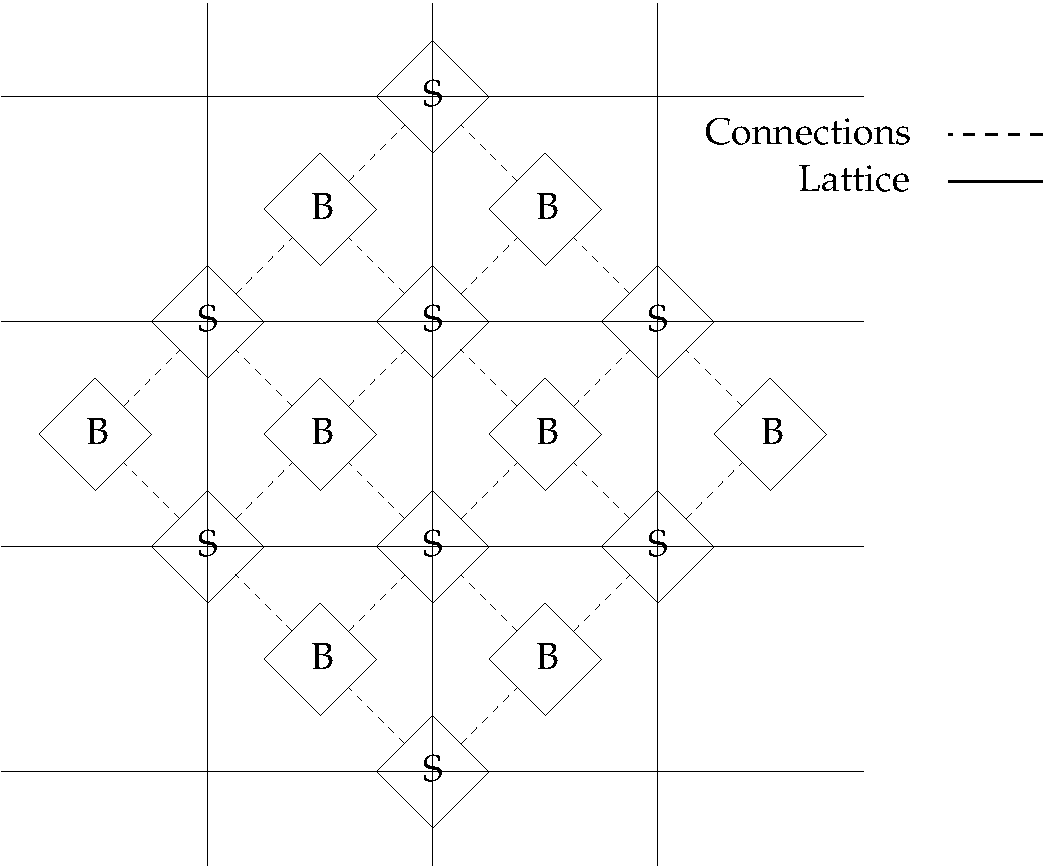
\includegraphics[height=4cm]{03-24-undergrad-project-presentation.figures/two-dim-lattice}}
  \end{center}
}

\subsection{System dynamics}
\frame
{
  \frametitle{System dynamics}
  \begin{itemize}
    \setlength{\itemsep}{\baselineskip}
  \item<1-> Buyers and Sellers
  \item<2-> Buyers just choose cheapest seller
  \item<3-> Sellers sell equally to all buyers
  \item<4-> Sellers die and are reborn stochastically
    (probability $\gamma$)
  \end{itemize}
}

\section{Expectations}

\subsection{Nash Equilibrium}
\frame
{
  \frametitle{Zero-dimensional Model}
  \begin{itemize}
    \setlength{\itemsep}{\baselineskip}
  \item<1-> Well understood (Nash, 1951)
  \item<2-> System moves to zero-profit equilbrium, ``Nash
    equilbrium''
  \item<3-> Does our model do the same?  Maybe
  \end{itemize}
}

\subsection{Mean Field Approach}

\frame 
{
  \frametitle{Can Expensive Shops Exist?}
  \begin{itemize}
    \setlength{\itemsep}{\baselineskip}
  \item<1-> If all shops are cheap, not enough demand---some die
  \item<2-> Dead sites allow expensive shops---competing
    against dead sites
  \item<3-> Can approach this by appealing to a mean field
    argument
  \end{itemize}
}

\frame
{
  \frametitle{Mean Field of Shops}
  \begin{itemize}
    \setlength{\itemsep}{\baselineskip}
  \item<1-> Equilibrium number of cheap shops (assuming all
    are cheap) is $N_c = N(1 - R\Gamma)$
  \item<2-> Postulate expensive shops
  \item<3-> Number of expensive shops is $N_e =
    N\frac{P_\alpha R\Gamma}{1 - R\Gamma}$.  $P_\alpha$ the
    probability of attracting $\alpha$ buyers
  \item<4-> Gives some idea of what to expect/test for
  \end{itemize}
}

\section{Results}

\subsection{One-dimensional Model}

\frame
{
  \frametitle{System Layout}
  \begin{itemize}
    \setlength{\itemsep}{\baselineskip}
  \item<1-> System on ring (periodic boundary conditions)
    \vspace{\baselineskip}
    \begin{center}
      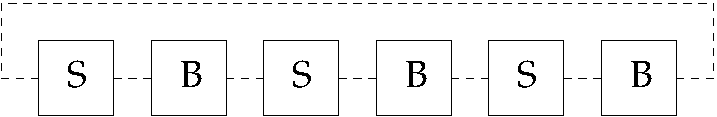
\includegraphics[width=6cm]{03-24-undergrad-project-presentation.figures/one-dim-lattice}
    \end{center}
  \item<2-> Twice as much demand as supply---if a shop
    attracts both buyers it can sate their consumerist desires
  \item<3-> Mean field approach says $N_c = 5830$ and $N_e = 1670$.
  \end{itemize}
}

\subsection{Equilibrium distribution}
\frame
{
  \frametitle{Equilibrium price distribution}
  \begin{minipage}{0.4\textwidth}
  \begin{itemize}
    \setlength{\itemsep}{\baselineskip}
    \item<1-> Mostly cheap shops, but some expensive ones
    \item<2-> Note peaks at around $0.125$ (marginal cost),
      $0.25$, $0.375$ and $0.5$
    \item<3-> Gives $N_c \approx 5100$ and $N_e \approx
      2400$---reasonable agreement with mean field predictions
    \end{itemize}
  \end{minipage}
  \begin{minipage}{0.5\textwidth}
    \begin{center}
      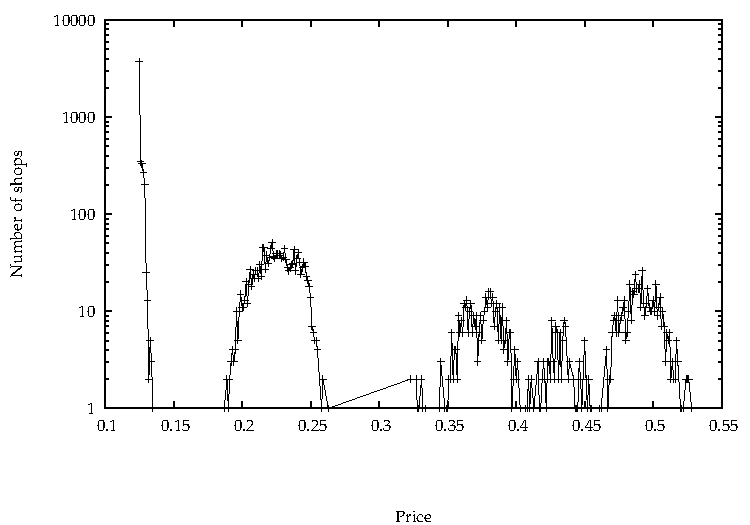
\includegraphics[width=6cm]{03-24-undergrad-project-presentation.figures/shop-price-projection-1}
    \end{center}%
  \end{minipage}
}

\subsection{Why structure?}
\frame
{
  \frametitle{Why peaks?}
  \begin{itemize}
    \setlength{\itemsep}{\baselineskip}
  \item<1-> Constant demand means that shops can predict it
  \item<2-> Surviving for non-integer number of game rounds
    not possible
  \item<3-> Gives peaks in prices at integer multiples of
    marginal cost
  \item<4-> Surviving for $2 \frac{1}{2}$ rounds has no
    advantage over surviving for $2$ rounds, but has the disadvantage
    that there are fewer shops to outcompete
  \item<5-> Not as clear cut as this, why?
  \end{itemize}
}


\subsection{Profits}

\frame
{
  \frametitle{Non-zero Profits}
  \begin{minipage}{0.4\textwidth}
    \begin{itemize}
      \setlength{\itemsep}{\baselineskip}
    \item<1-> Profits not zero for all prices
    \item<2-> Large profits correspond to shops in price bands
    \item<3-> Why?  Competition within price bands favours
      cheaper shops.  Equilibrium mechanism keeps number of shops
      constant
    \end{itemize}
  \end{minipage}
  \begin{minipage}{0.5\textwidth}
    \only<1>{%
      \begin{center}
        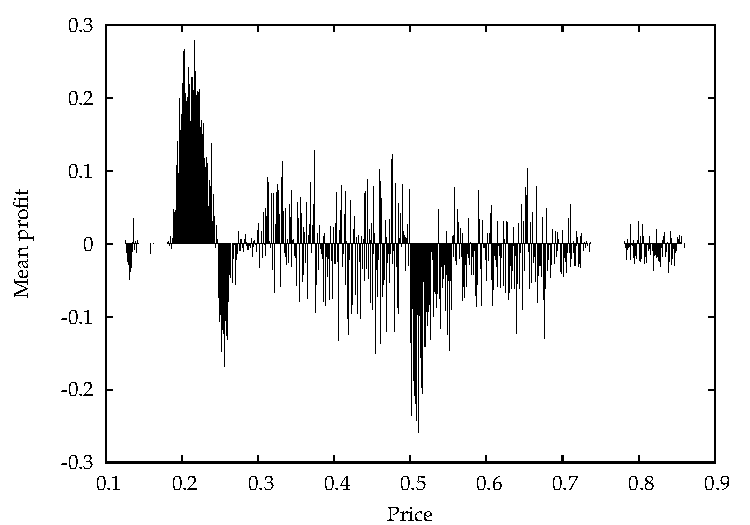
\includegraphics[width=6cm]{03-24-undergrad-project-presentation.figures/time-average-profit}
      \end{center}%
    } \only<2>{%
      \begin{center}
        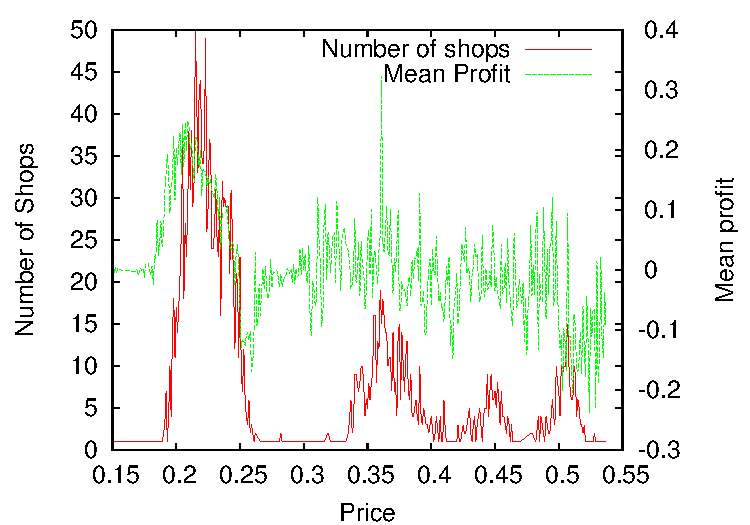
\includegraphics[width=6cm]{03-24-undergrad-project-presentation.figures/price-profit}
      \end{center}%
    } \only<3>{%
      \begin{center}
        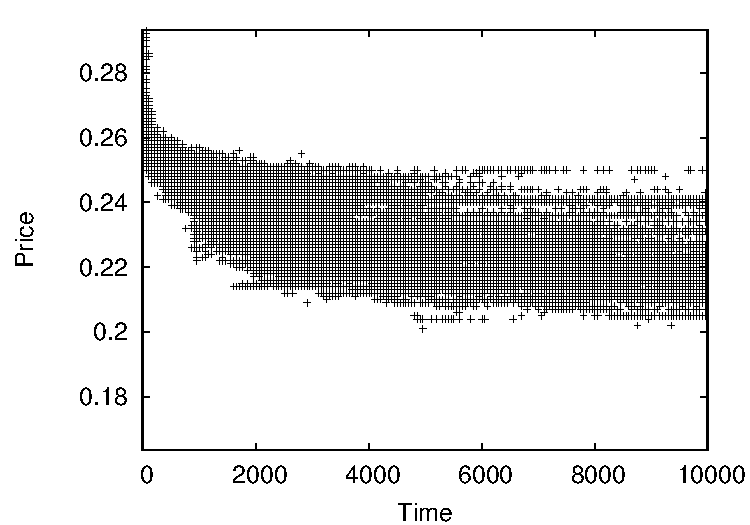
\includegraphics[width=6cm]{03-24-undergrad-project-presentation.figures/price-time-equi}
      \end{center}%
    }
  \end{minipage}
}



\frame
{
  \frametitle{Random Demand}
  \begin{minipage}{0.4\textwidth}
    \begin{itemize}
      \setlength{\itemsep}{\baselineskip}
    \item<1-> Expect no peaks, since shops cannot predict local demand
    \item<2-> This is the case, except for high-priced shops
    \item<3-> High priced-shops still peak---can survive for long
      enough that local demand is constant
    \end{itemize}
  \end{minipage}
  \begin{minipage}{0.5\textwidth}
    \only<2->{%
      \begin{center}
        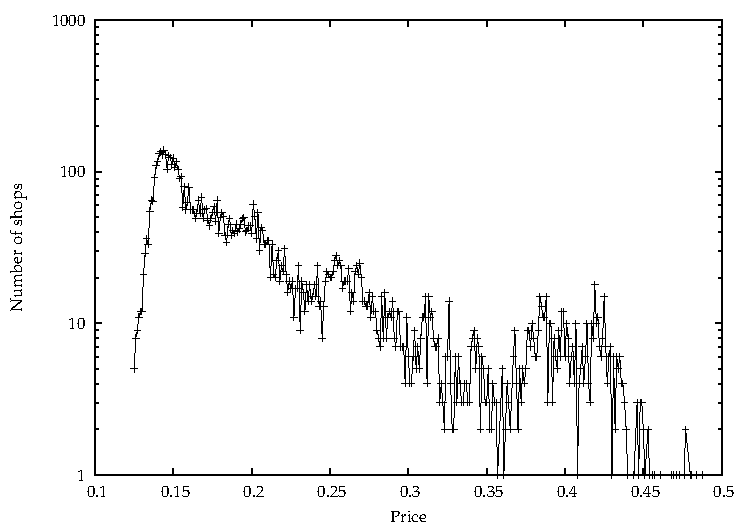
\includegraphics[height=4cm]{03-24-undergrad-project-presentation.figures/shop-price-projection-2}
      \end{center}%
    }
  \end{minipage}
}

\subsection{Lifetimes}
\frame
{
  \frametitle{Lifetimes of Shops}
  \begin{minipage}{0.4\textwidth}
    \begin{itemize}
      \setlength{\itemsep}{\baselineskip}
    \item<1-> No death built into model
    \item<2-> All shops die nonetheless (although some are nearly as
      old as system)
    \item<3-> Closer inspection shows us which
    \end{itemize}
  \end{minipage}
  \begin{minipage}{0.5\textwidth}
    \only<2>{%
      \begin{center}
        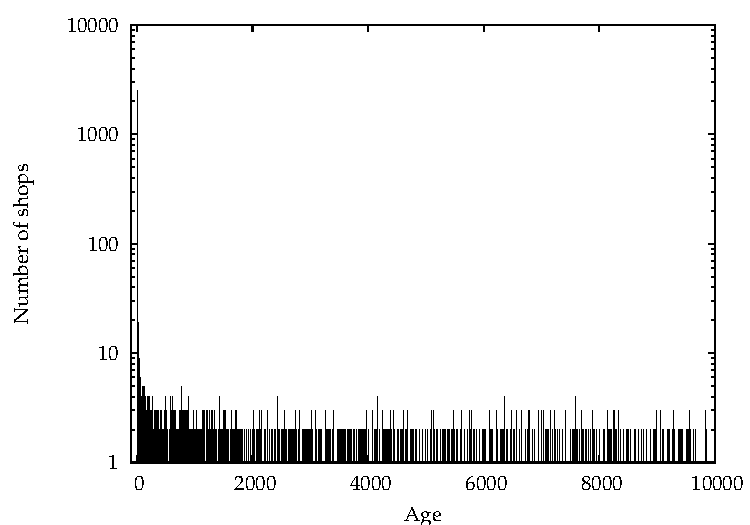
\includegraphics[width=6cm]{03-24-undergrad-project-presentation.figures/age-number}
      \end{center}%
    } \only<3>{%
      \begin{center}
        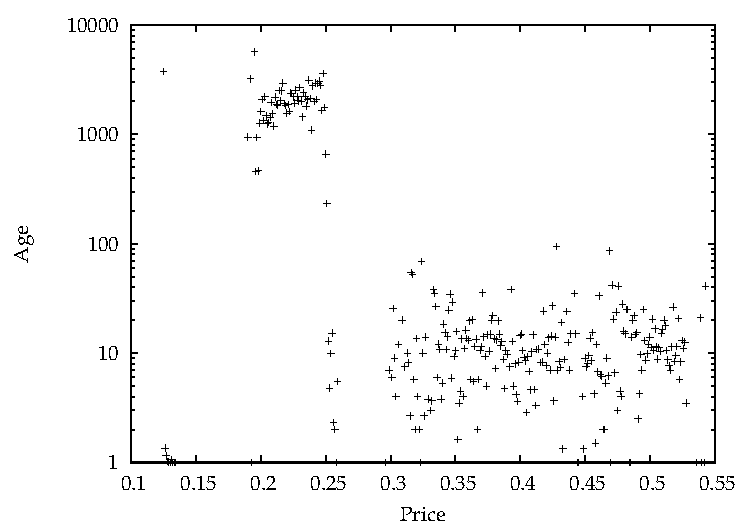
\includegraphics[width=6cm]{03-24-undergrad-project-presentation.figures/age-price}
      \end{center}%
    }
  \end{minipage}
}

\section{Conclusions}

\frame
{
  \frametitle{What We Have Achieved}
  \begin{itemize}
    \setlength{\itemsep}{\baselineskip}
  \item<1-> Simple Economic model---produces results with analogs in
    real-world phenomena
  \item<2-> Simple enough that at least some features can be explained
    analytically---appeals to Economists
  \item<3-> Many features unexplained
  \end{itemize}
}

\frame
{
  \frametitle{The Trouble With Simulations}
  \begin{itemize}
    \setlength{\itemsep}{\baselineskip}
  \item<1-> Still far less complex than real world
  \item<2-> Difficult to explain some phenomena without wild
    handwaving
  \item<3-> Still a long way from being able to tell a shopkeeper what
    price to charge
  \end{itemize}
}
\end{document}
